%\pagenumbering{arabic}
%\setcounter{page}{1}
\setcounter{chapter}{9}
\chapter{Two Sample Confidence Interval}
%\index{Introduction}
%\label{sec.matrix}
%start relabeling as 2.1 etc
%\pagestyle{myheadings}  \markboth{\ref{sec.matrix}.
%\titleref{sec.matrix}}{}
%\setcounter{equation}{0}

We have discussed three distinct types of one sample confidence interval. Now, let's keep moving forward to see how confidence interval works for two sample. The aim of one sample confidence interval is giving a range of numbers to estimate population mean or proportion with a certain percentage of confidence. For two samples, the aim is comparing with sample has a relatively larger or smaller population mean or proportion with a certain percentage of confidence.

\section{Two Sample Confidence Interval on a Difference of Mean}

Suppose we are interested in the final mark of MAT135 from the same semester but with different campuses at the University of Toronto (let's use UTSG and UTM as the two independent population groups). We want to know which campus has a relatively higher average score, the question is: how do we determine that? It is going to be complicated if we proceed with the study directly by determining the sum of everyone's final marks and calculating the average for the two campuses. Similarly, as one sample confidence interval, we can select two groups of random sample from the two campuses (one group per each campus), and then calculate each sample mean. Finally, we apply a confidence interval to approximate which population has a higher mean (or average).\\

\textbf{Two Sample Confidence Interval for Two Independent Groups of Population}

We are going to introduce several definitions because two sample confidence interval has distinct cases. You need to be able to identify which exact case you are facing from given information. If you know how to solve one sample confidence interval, then two sample confidence interval is going to be easy, because all the techniques from one sample confidence interval are still usable.\\

\textbf{Case 1:} Two sample confidence interval with given population variance for both groups.\\

\begin{definition}[Two sample confidence interval with given population variances]
Suppose we are given the population variance for both two independent groups of population. The confidence interval of $\mu_1 - \mu_2$ (difference of mean between population group 1 and 2) is given by the following: \[ (\bar{x}_{1} - \bar{x}_{2})  \pm z_{\small\alpha/2} \cdot \sqrt{ \frac{\sigma_1^2}{n_1} + \frac{\sigma_2^2}{n_2}}.\]
For $\sigma_1^2$, which is population variance of population group 1; $n_1$ is the sample size chosen form population group 1. Similarly for $\sigma_2^2$, which is population variance of population group 2; $n_2$ is the sample size chosen form population group 2.
\end{definition}

Additionally, case 1 is a bit unrealistic with other cases because the population variance ($\sigma^2$) from both groups are rare to know.\\

\textbf{Case 2:} Two sample confidence interval with equal unknown population variance\\

Ideally, we have all the information about population variance from two chosen samples. However, that case does not usually happen. We may face the case with unknown variance.

\begin{definition}
Suppose that the chosen two independent samples have same unknown population variance. Then the two sample confidence interval for $\mu_1 - \mu_2$ is given by the following: $$(\bar{x}_1 - \bar{x}_2)  \pm  t_{n_1+n_2-2; \alpha/2} \cdot s_p \cdot \sqrt{\frac{1}{n_1} + \frac{1}{n_2}}.$$
In this case, $n_1$ and $n_2$ are sample size from the two chosen samples respectively; $s_p$ is aggregated variance of both samples combined which accommodates samples of different sizes.
Additionally, $s_p$ is called pooled standard deviation which is calculated by the following equation: $$s_p^2 = \frac{(n_1-1) \cdot s_1^2 + (n_2-1) \cdot s_2^2 }{n_1+n_2-2},$$
where $s_1^2$ and $s_2^2$ are sample variance of the two chosen samples respectively.\\
Then we take the square root $s_p = \sqrt{s_p^2}$ to get pooled standard deviation.
\end{definition}

Alternatively, we can write the equation for two sample confidence interval with equal unknown variance as: $$(\bar{x}_1 - \bar{x}_2)  \pm  t_{n_1+n_2-2; \alpha/2} \cdot \sqrt{s_p^2(\frac{1}{n_1} + \frac{1}{n_2})}, \text{ which is same as the one above.}$$

\textbf{Pooled Variance and Standard Deviation}

In statistics, pooled variance (also known as combined variance, composite variance, or overall variance) is a method to calculate such a value in order to estimate variance between several distinct populations. The mean of each population may or may not be the same, but the variance of these populations are same. Pooled standard deviation does similar thing, we use that value to estimate standard deviation instead of variance.\\

\textbf{Case 3:} Two sample confidence interval with unequal unknown population variance\\

At this point, you may wonder that what if the population variance is both unequal and unknown? Does two sample confidence interval still doable in this case? The answer is: Yes. We can still proceed with two sample confidence interval.

\begin{definition}
Suppose that our chosen two independent samples with unequal and unknown population variance, then the confidence interval for $\mu_1 - \mu_2$ is given by: $$(\bar{x}_1 - \bar{x}_2)  \pm t_{df; \alpha/2} \cdot \sqrt{\frac{s_1^2}{n_1} + \frac{s_2^2}{n_2}}, \text{ where: $df = min(n_1-1, n_2-1)$.}$$
Moreover, $s_1^2$ and $s_2^2$ are sample variance of the two chosen groups; and $n_1$, $n_2$ are the sample size of the two chosen groups respectively.
\end{definition}

\textbf{Visualization of Two Sample Confidence Interval}

Only with the equation seems hard to understand, the following number line helps you to visualize what we try to indicate:
\begin{center}
\begin{figure}[h!]
\centering
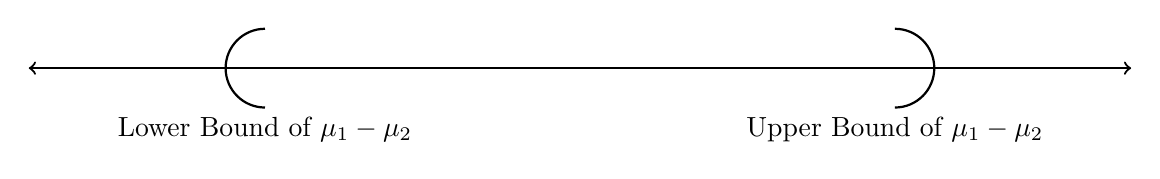
\begin{tikzpicture}
  \draw[<->, thick] (-7,0) -- (7,0);
  \draw[thick] (-4,-0.5) arc (270:90:0.5);
  \node[below] at (-4,-0.5) {Lower Bound of $\mu_1 - \mu_2$};
  \draw[thick] (4,0.5) arc (90:-90:0.5);
  \node[below] at (4,-0.5) {Upper Bound of $\mu_1 - \mu_2$};
\end{tikzpicture}
\caption{Visualization of two-sample confidence interval (Case 1, 2, 3)}
\end{figure}
\end{center}

Earlier in this chapter we said that two sample confidence interval aims to compare the mean between two populations. The number line above shows the result of difference of means between the two populations. Now, the question is, how do we know which population has a relatively larger mean? While, we can summarize it from that number line, with different cases:

\textbf{1. $\mu_1 < \mu_2$:}

\begin{center}
\begin{figure}[h!]
\centering
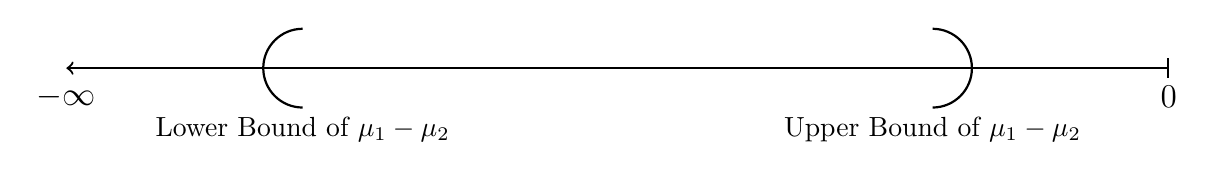
\begin{tikzpicture}
  \draw[<-|, thick] (-7,0) -- (7,0);
  \draw[thick] (-4,-0.5) arc (270:90:0.5);
  \node[below] at (-4,-0.5) {Lower Bound of $\mu_1 - \mu_2$};
  \draw[thick] (4,0.5) arc (90:-90:0.5);
  \node[below] at (4,-0.5) {Upper Bound of $\mu_1 - \mu_2$};
  \node[below] at (-7, -0.1) {\large$-\infty$};
  \node[below] at (7, -0.1) {\large$0$};
\end{tikzpicture}
\caption{Visualization of the case when $\mu_1 < \mu_2$}
\end{figure}
\end{center}

Now, we know that the difference between $\mu_1 < \mu_2$ lies on the negative side on the number line, such that: $\mu_1 - \mu_2 < 0$. Hence, by solving the inequality above we get: $\mu_1 < \mu_2$ trivially.

\textbf{2. $\mu_1 > \mu_2$:}

\begin{center}
\begin{figure}[h!]
\centering
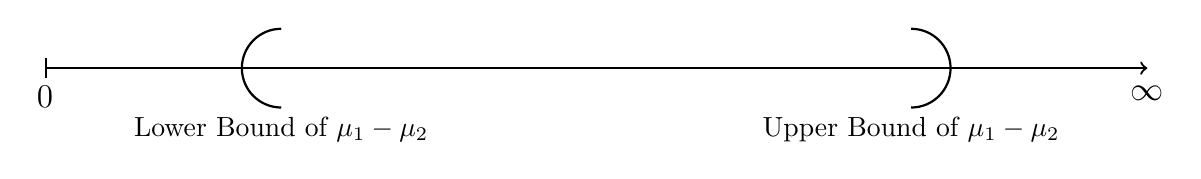
\begin{tikzpicture}
  \draw[|->, thick] (-7,0) -- (7,0);
  \draw[thick] (-4,-0.5) arc (270:90:0.5);
  \node[below] at (-4,-0.5) {Lower Bound of $\mu_1 - \mu_2$};
  \draw[thick] (4,0.5) arc (90:-90:0.5);
  \node[below] at (4,-0.5) {Upper Bound of $\mu_1 - \mu_2$};
  \node[below] at (-7, -0.1) {\large$0$};
  \node[below] at (7, -0.1) {\large$\infty$};
\end{tikzpicture}
\caption{Visualization of the case when $\mu_1 > \mu_2$}
\end{figure}
\end{center}

Similarly as the case above, we know that $\mu_1 - \mu_2 > 0$, by observing the number line. Thus, we have: $\mu_1 > \mu_2$.

\textbf{3. $\mu_1 = \mu_2$:}

\begin{center}
\begin{figure}[h!]
\centering
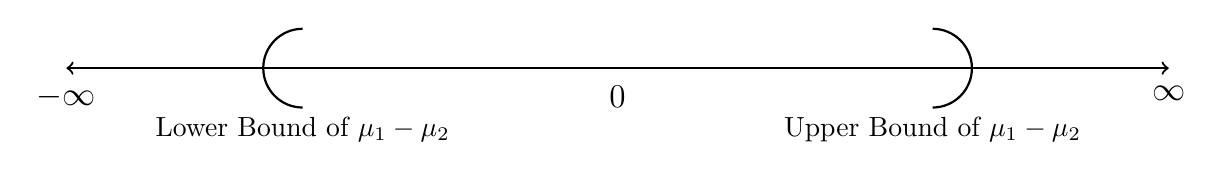
\begin{tikzpicture}
  \draw[<->, thick] (-7,0) -- (7,0);
  \draw[thick] (-4,-0.5) arc (270:90:0.5);
  \node[below] at (-4,-0.5) {Lower Bound of $\mu_1 - \mu_2$};
  \draw[thick] (4,0.5) arc (90:-90:0.5);
  \node[below] at (4,-0.5) {Upper Bound of $\mu_1 - \mu_2$};
  \node[below] at (0, -0.1) {\large$0$};
  \node[below] at (7, -0.1) {\large$\infty$};
  \node[below] at (-7, -0.1) {\large$-\infty$};
\end{tikzpicture}
\caption{Visualization of the case when $\mu_1 = \mu_2$}
\end{figure}
\end{center}

However, 0 is an element in the range of the difference between $\mu_1 - \mu_2$, such that there is a chance when the two means could be same. Hence, we conclude that $\mu_1 = \mu_2$ in this case. While, if you prefer to use $\mu_2 - \mu_1$, this strategy is going to work as well. Just simply following the same steps, you will get the same conclusion.\\

\textbf{Conditions of Two Sample Confidence Interval}

Same as all previous confidence intervals, we still need several conditions that guarantee the validity two sample confidence interval:

\begin{itemize}
	\item 1. The two chosen sample is required to be independent and random;
	\item 2. If both sample size are small (both $n_1 < 30$ and $n_2 < 30$), then both sample should be from normal population;
	\item 3. If one of the sample has a small size (either $n_1 < 30$ or $n_2 < 30$), then the smaller sample must be from a normal population;
\end{itemize}

Note that if both $n_1 \ge 30$ and $n_2 \ge 30$, then normality assumption is not required by the Central Limit Theorem.\\

\textbf{Example (Comparing Two Population Means Managerial Success Indexes for Two Groups)}

\begin{example}
Behavioural researchers have developed an index designed to measure managerial success. The index (measured on a 100- point scale) is based on the manager’s length of time in the organization and their level within the term; the higher the index, the more successful the manager. Suppose a researcher wants to compare the average index for the two groups of managers at a large manufacturing plant. Managers in group 1 engage in high volume of interactions with people outside the managers’ work unit (such interaction include p hone and face-to-face meetings with customers and suppliers, outside meetings, and public relation work). Managers in group 2 rarely interact with people outside their work unit. Independent random samples of 12 and 15 managers are selected from groups 1 and 2, respectively, and success index of each is recorded.\\
Comparing Two Population Means Managerial Success Indexes for Two Group (With Equal Variances Assumed) Note: The response variable is “Managerial Success Indexes”.

Managerial success indexes is a continuous quantitative variable,

measured on100-point scale.

The explanatory variable is “Type of group”.

Type of group (Group 1: Interaction with outsiders, Group 2: Fewer interactions) is a nominal categorical variable.

Let's use R-code to demonstrate this example. The following lines of code helps you to get started.

\begin{tcolorbox}[colback=gray!10, colframe=gray!50, arc=2mm]
\begin{verbatim}
# Importing data file into R;

success=read.csv(file="success.csv",header=TRUE);

# Getting names of variables;

names(success);

# Seeing first few observations;

head(success);

# Attaching data file; attach(success);
\end{verbatim}
\end{tcolorbox}

Now, you will get the following table by running the code above from R-studio.

\begin{tcolorbox}[colback=gray!10, colframe=gray!50, arc=2mm]
\begin{verbatim}
## [1] "Success_Index" "Group" 
## Success_Index Group 
## 1 65 1 
## 2 66 1 
## 3 58 1 
## 4 70 1 
## 5 78 1 
## 6 53 1
\end{verbatim}
\end{tcolorbox}

Then, we use R-studio to obtain some descriptive statistics.

\begin{tcolorbox}[colback=gray!10, colframe=gray!50, arc=2mm]
\begin{verbatim}
##	.group  min    Q1 median    Q3 max     mean       sd  n
## 1 		 1   53 62.25   65.5 69.25  78 65.33333 6.610368 12
## 2 		 2   34 42.50   50.0 54.50  68 49.46667 9.334014 15
## 	missing
## 1 		   0
## 2 		   0
\end{verbatim}
\end{tcolorbox}

Note that: Group 1 = “interaction with outsiders” and Group 2 = “fewer interactions”. Then, we can proceed with two sample confidence interval.

\begin{tcolorbox}[colback=gray!10, colframe=gray!50, arc=2mm]
\begin{verbatim}
# 95\% CI for the difference between means; 
# equal variances is assumed;

t.test(Success_Index~Group, 
var.equal=TRUE, conf.level=0.95)$conf.int;
\end{verbatim}
\end{tcolorbox}

Finally, the output is:

\begin{tcolorbox}[colback=gray!10, colframe=gray!50, arc=2mm]
\begin{verbatim}
## [1] 9.288254 22.445079 
## attr(,"conf.level") 
## [1] 0.95
\end{verbatim}
\end{tcolorbox}

Therefore, We are 95\% confident that the mean success index is between 9.28 and 22.44 points higher for group 1 than group 2.
\end{example}

\section{Two Sample Confidence Interval on Paired Data}

It seems like two sample confidence interval only works on two independent samples, however what about two dependent samples? Suppose we are interested the growth of height from several distinct elementary students. We measure their height recently, then we will do it another time with five years later. The question is: how are we going to proceed with two confidence interval? While, the answer is yes. We are able to do so by constructing two sample confidence interval, but with a different strategy. Now, let's introduce two sample confidence interval with paired data:

\begin{center}
\begin{figure}[h!]
\centering
\begin{tabular}{ c c c c }
 Sample Units & Measurement 1 ($M_1$) & Measurement 2 ($M_2$) & Difference ($M_2 - M_1$ or $M_1 - M_2$)\\ 
 1 & $x_{11}$ & $x_{12}$ & $x_{d1} = x_{12} -  x_{11}$\\  
 2 & $x_{21}$ & $x_{22}$ & $x_{d2} = x_{22} -  x_{21}$\\
 3 & $x_{31}$ & $x_{32}$ & $x_{d2} = x_{32} -  x_{31}$\\
 ......\\
 n & $x_{n1}$ & $x_{n2}$ & $x_{dn} = x_{n2} -  x_{n1}$\\
\end{tabular}
\caption{A table of paired data}
\end{figure}
\end{center}

The table shows how to get a paired data. The first column on the left is the sample size, the second column records the first time of measurement of objects, the third column records the second time of measurement of the same objects, the last column on the right is the difference between the second and the first measurement ($M_2 - M_1$). Then we can use the fourth column to get the mean value, sample variance and sample standard deviation of the difference. Now, let's begin with the proper definition:

\begin{definition}[Two Sample Confidence Interval on Paired Data]
Suppose we have two samples that are dependent with each other, the confidence interval on paired data's mean ($\mu_d$) is given by: \[ \bar{x}_d  \pm t_{n-1, \alpha/2} \cdot \frac{s_d}{\sqrt{n}}.\]
In this case, the reference distribution is t-distribution with $n-1$ degrees of freedom (sample size minus $1$), $\bar{x}_d$ represents the sample mean of difference between the two measurements on the paired data, $s_d$ is the sample standard deviation of difference between the two measurements.
\end{definition}

Note that: two sample confidence interval on paired data is to calculate a range of number on \textbf{the mean of difference between the two measurement}. Then, we can continue our analysis about the data.\\

\textbf{Visualization of Two Sample Confidence Interval on Paired Data}

Next, we need to state our final conclusion from the result of two sample confidence interval on paired data. Again, let's construct a number line for each case.

\textbf{1. $\bar{M}_1 < \bar{M}_2$:}

\begin{center}
\begin{figure}[H]
\centering
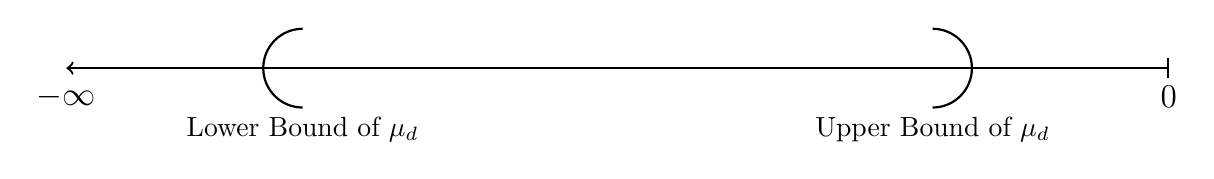
\begin{tikzpicture}
  \draw[<-|, thick] (-7,0) -- (7,0);
  \draw[thick] (-4,-0.5) arc (270:90:0.5);
  \node[below] at (-4,-0.5) {Lower Bound of $\mu_d$};
  \draw[thick] (4,0.5) arc (90:-90:0.5);
  \node[below] at (4,-0.5) {Upper Bound of $\mu_d$};
  \node[below] at (-7, -0.1) {\large$-\infty$};
  \node[below] at (7, -0.1) {\large$0$};
\end{tikzpicture}
\caption{Visualization of the case when $\bar{M}_1 < \bar{M}_2$}
\end{figure}
\end{center}

From the number line above, we know that the result of $\mu_d$ lies only in the negative side of the number line, also we use $M_1 - M_2$ to get the difference data then calculate the average of difference data. Now, we have: $\bar{M}_1 - \bar{M}_2 = \mu_d < 0$. Hence, we conclude that $\bar{M}_1 < \bar{M}_2.$

\textbf{2. $\bar{M}_1 > \bar{M}_2$:}

\begin{center}
\begin{figure}[H]
\centering
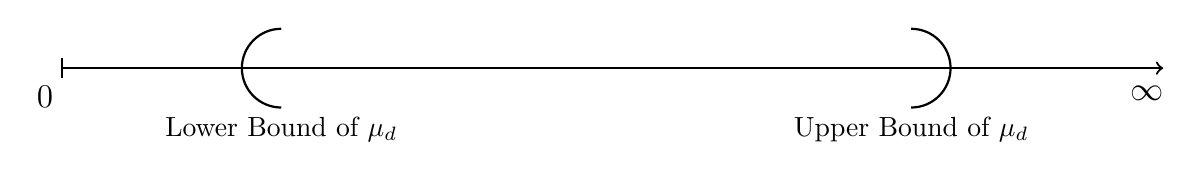
\begin{tikzpicture}
  \draw[|->, thick] (-6.8,0) -- (7.2,0);
  \draw[thick] (-4,-0.5) arc (270:90:0.5);
  \node[below] at (-4,-0.5) {Lower Bound of $\mu_d$};
  \draw[thick] (4,0.5) arc (90:-90:0.5);
  \node[below] at (4,-0.5) {Upper Bound of $\mu_d$};
  \node[below] at (-7, -0.1) {\large$0$};
  \node[below] at (7, -0.1) {\large$\infty$};
\end{tikzpicture}
\caption{Visualization of the case when $\bar{M}_1 > \bar{M}_2$}
\end{figure}
\end{center}

From the number line above, we know that the result of $\mu_d$ lies only in the positive side of the number line, also we use $M_1 - M_2$ to get the difference data then calculate the average of difference data. Now, we have: $\bar{M}_1 - \bar{M}_2 = \mu_d > 0$. Hence, we conclude that $\bar{M}_1 > \bar{M}_2.$

\textbf{3. $\bar{M}_1 = \bar{M}_2$:}

\begin{center}
\begin{figure}[H]
\centering
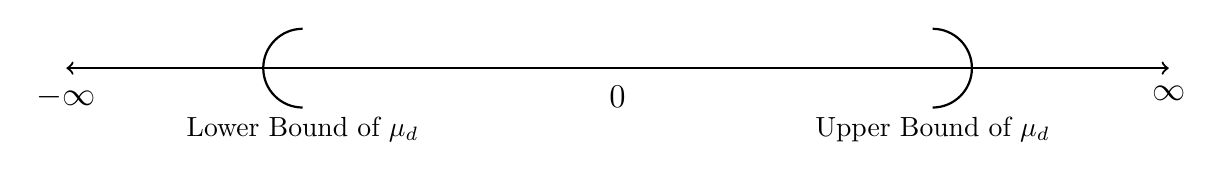
\begin{tikzpicture}
  \draw[<->, thick] (-7,0) -- (7,0);
  \draw[thick] (-4,-0.5) arc (270:90:0.5);
  \node[below] at (-4,-0.5) {Lower Bound of $\mu_d$};
  \draw[thick] (4,0.5) arc (90:-90:0.5);
  \node[below] at (4,-0.5) {Upper Bound of $\mu_d$};
  \node[below] at (0, -0.1) {\large$0$};
  \node[below] at (7, -0.1) {\large$\infty$};
  \node[below] at (-7, -0.1) {\large$-\infty$};
\end{tikzpicture}
\caption{Visualization of the case when $\bar{M}_1 = \bar{M}_2$}
\end{figure}
\end{center}

While, 0 is included in the range of $\mu_d$, then there is a chance that $\bar{M}_1 - \bar{M_2} = \mu_d = 0.$ Hence, we conclude that $\bar{M}_1 = \bar{M}_2$.\\

\textbf{Conditions of Two Sample Confidence Interval on Paired Data}

We need the following conditions to make sure the validity of two sample confidence interval on paired data:

\begin{itemize}
	\item 1. Units are independent (measurements are dependent on each unit)
	\item 2. Units must be random sample
	\item 3. If we have a small sample ($n < 30$), then the population of difference should be normal (no restrictions on large samples).
\end{itemize}

Also, note that two sample confidence interval on paired data can only be applied with two dependent groups of data. For independent groups of data, you need to refer chapter 10.1.

\section{Two Sample Confidence Interval on Proportions}

Furthermore, two sample confidence intervals can approximate the proportion as well. Suppose we are interested in the proportion of left-handed students in UTSG and UTM, and we are asked to find the campus that has a relatively larger proportion of left-handed students. To begin with this task, it is impossible to complete it directly by calculation, due to its complexity and high workload. We can use select two independent groups (one group from each campus), then apply two sample confidence interval to approximate which campus has a larger proportion.\\

It may still be difficult to understand, now let's begin with figures:

\begin{center}
\begin{figure}[h!]
\centering

\begin{tikzpicture}
  \draw[fill=blue, line width=2pt] ( -3, 0) circle (2cm);
  \draw[fill=red, line width=2pt] ( 3, 0) circle (2cm);
\end{tikzpicture}
\caption{Visualization of two population of all students from UTSG (left) and UTM (right)}
\end{figure}
\end{center}

This figure represents the population of all students from two campuses. To begin with our task (find the proportion of left-handed students), we can select a group of random sample from each campus:

\begin{center}
\begin{figure}[h!]
\centering
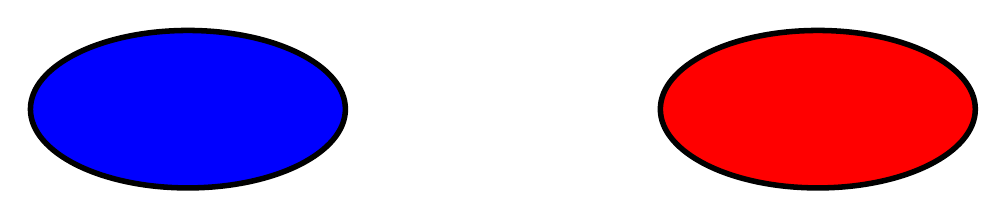
\begin{tikzpicture}
  % Blue ellipse on the left
  \draw[fill=blue, line width=2pt] (-4, 0) ellipse [x radius=2cm, y radius=1cm];

  % Red ellipse on the right
  \draw[fill=red, line width=2pt] (4, 0) ellipse [x radius=2cm, y radius=1cm];
\end{tikzpicture}
\caption{Visualization of two selected random sample from UTSG (left) and UTM (right)}
\end{figure}
\end{center}

As you can see, we have chosen our random sample from each campus with sample size $n_1$ and $n_2$, respectively. Now we need estimators to construct our confidence interval: $\hat{p}_1$ and $\hat{p}_2$. Those are the proportion of left-handed students from each random sample respectively. Since we have all the information we need, now we can apply our confidence interval from the two random sample.

\begin{definition}[Two Sample Confidence Interval on Proportions]
Draw an SRS of size $n_1$ from a population having proportion $p_1$ of successes and draw an independent SRS of size $n_2$ from another population having proportion $p_2$ of successes. When $n_1$ and $n_2$ are large, an approximate level C confidence interval for $p_1 - p_2$ is given by: \[ (\hat{p}_1 - \hat{p}_2)  \pm z_{\alpha/2} \cdot \sqrt{ \frac{\hat{p}_1(1-\hat{p}_1)}{n_1} + \frac{\hat{p}_2(1-\hat{p}_2)}{n_2}}.\]
Now, $n_1$ and $n_2$ are sample size of selected random sample from each population; $\hat{p}_1$ and $\hat{p}_2$ are the proportion of success of each selected random sample respectively.
\end{definition}

Note that, $\hat{p}_1 = \frac{\text{number of successes in random sample 1}}{n_1}$ and $\hat{p}_2 = \frac{\text{number of successes in random sample 2}}{n_2}$.

\textbf{Visualization of $p_1 - p_2$}

Similarly as confidence interval on independent and dependent data, we are going to provide number lines, in order to help you to visualize the result easily.

\textbf{1. $p_1 > p_2$:}

\begin{center}
\begin{figure}[h!]
\centering
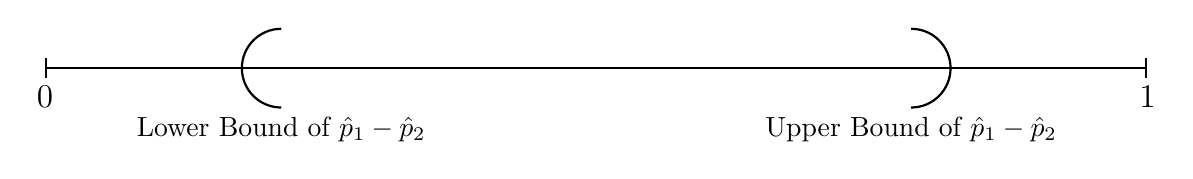
\begin{tikzpicture}
  \draw[|-|, thick] (-7,0) -- (7,0);
  \draw[thick] (-4,-0.5) arc (270:90:0.5);
  \node[below] at (-4,-0.5) {Lower Bound of $\hat{p}_1 - \hat{p}_2$};
  \draw[thick] (4,0.5) arc (90:-90:0.5);
  \node[below] at (4,-0.5) {Upper Bound of $\hat{p}_1 - \hat{p}_2$};
  \node[below] at (7, -0.1) {\large$1$};
  \node[below] at (-7, -0.1) {\large$0$};
\end{tikzpicture}
\caption{Visualization of the case when $p_1 > p_2$}
\end{figure}
\end{center}

From the number line, the result of $\hat{p}_1 - \hat{p}_2$ lies only on the positive side, such that $\hat{p}_1 - \hat{p}_2 > 0$. Hence, $\hat{p}_1 > \hat{p}_2$. Note that proportion is a number between $0$ and $1$, such that the difference of two proportions only between $-1$ and $1$.

\textbf{2. $\hat{p}_1 < \hat{p}_2$}

\begin{center}
\begin{figure}[h!]
\centering
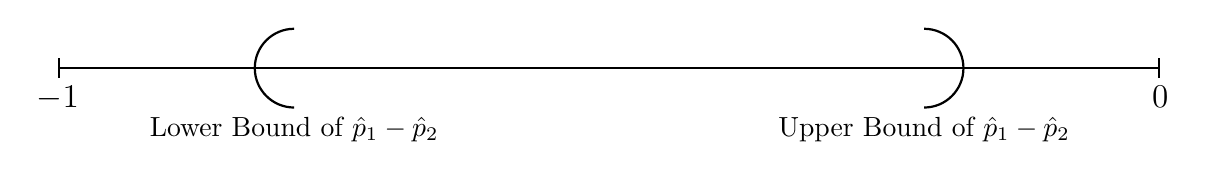
\begin{tikzpicture}
  \draw[|-|, thick] (-7,0) -- (7,0);
  \draw[thick] (-4,-0.5) arc (270:90:0.5);
  \node[below] at (-4,-0.5) {Lower Bound of $\hat{p}_1 - \hat{p}_2$};
  \draw[thick] (4,0.5) arc (90:-90:0.5);
  \node[below] at (4,-0.5) {Upper Bound of $\hat{p}_1 - \hat{p}_2$};
  \node[below] at (7, -0.1) {\large$0$};
  \node[below] at (-7, -0.1) {\large$-1$};
\end{tikzpicture}
\caption{Visualization of the case when $p_1 < p_2$}
\end{figure}
\end{center}

Now, the result of $\hat{p}_1 - \hat{p}_2$ lies only on the positive side, such that $\hat{p}_1 - \hat{p}_2 < 0$. Hence, $\hat{p}_1 < \hat{p}_2$.

\textbf{3. $\hat{p}_1 = \hat{p}_2$}

\begin{center}
\begin{figure}[h!]
\centering
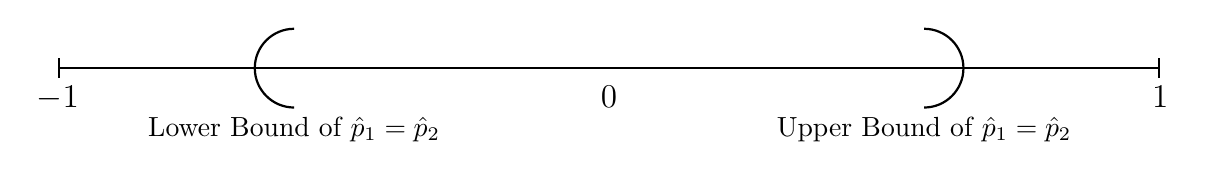
\begin{tikzpicture}
  \draw[|-|, thick] (-7,0) -- (7,0);
  \draw[thick] (-4,-0.5) arc (270:90:0.5);
  \node[below] at (-4,-0.5) {Lower Bound of $\hat{p}_1 = \hat{p}_2$};
  \draw[thick] (4,0.5) arc (90:-90:0.5);
  \node[below] at (4,-0.5) {Upper Bound of $\hat{p}_1 = \hat{p}_2$};
  \node[below] at (0, -0.1) {\large$0$};
  \node[below] at (7, -0.1) {\large$1$};
  \node[below] at (-7, -0.1) {\large$-1$};
\end{tikzpicture}
\caption{Visualization of the case when $\hat{p}_1 = \hat{p}_2$}
\end{figure}
\end{center}

In this case, $0$ lies in the range of $\hat{p}_1 - \hat{p}_2$, such that there is a chance when $\hat{p}_1 - \hat{p}_2 = 0$. Hence, we conclude that: $\hat{p}_1 = \hat{p}_2$.\\

\textbf{Conditions of Two Sample Confidence Interval on Proportion}

\begin{itemize}
	\item 1. Randomization Condition: The data in each group should be drawn independently and at random from a population or generated b y a completely randomized designed experiment.
	\item 2. The $10\%$ Condition: If the data are sampled without replacement, the sample should not exceed $10\%$ of the population. If samples are bigger than $10\%$ of the target population, random draws are no longer approximately independent.
	\item 3. Independent Groups Assumption: The two groups we are comparing must be independent from each other.
	\item 4. Sample size requirement: both selected sample size must greater than $70$.
\end{itemize}

\section{Two Sample Confidence Interval on Variances}

Confidence interval is a strong technique in inferential statistics, we have discussed its application on population mean, proportion and dependent data. Now, let's move on to variance.\\

One simple method involves just looking at two sample variances. Logically, if two population variances are equal, then the two sample variances should be very similar. When the two sample variances are reasonably close, you can be reasonably confident that the homogeneity assumption is satisfied and proceed with, for example, Student t-interval. However, when one sample variance is three or four times larger than the other, then there is reason for a concern. The common statistical procedure for comparing population variances $\sigma_1^2$ and $\sigma_2^2$ makes an inference about the ratio of $(\sigma_1^2)/(\sigma_2^2)$.\\

To make an inference about the ratio of $(\sigma_1^2)/(\sigma_2^2)$ we collect sample data and use the ratio of the sample variances $(\sigma_1^2)/(\sigma_2^2)$.

At this point, let's derive the confidence interval. We know that: $\frac{s_1^2/\sigma_1^2}{s_2^2/\sigma_2^2} \sim F_{n_1-1, n_2 -1}$. Then, we can construct our confidence interval as:
	\[P[F_{n_1-1, n_2 -1; 1-\alpha/2} < \frac{s_1^2/\sigma_1^2}{s_2^2/\sigma_2^2} < F_{n_1-1, n_2 -1; \alpha/2}]  = 1 -\alpha.\]
Now, the reference distribution of this confidence interval is F-distribution with $n_1 - 1$ and $n_2 -1$ degrees of freedom, leaving areas of $1 - \alpha/2$ and $\alpha/2$, respectively, to the right. Rearranging gives us:
	\[P[\frac{s_1^2}{s_2^2} \cdot \frac{1}{F_{n_1-1, n_2 -1; \alpha/2}} < \frac{\sigma_1^2}{\sigma_2^2} < \frac{s_1^2}{s_2^2} \cdot \frac{1}{F_{n_1-1, n_2 -1; 1-\alpha/2}}] = 1 -\alpha.\]
Using the face that $F_{n_1-1,n_2-1; 1 - \alpha/2} = \frac{1}{F_{n_2-1,n_1-1; \alpha/2}}$, we have:
	\[ P[\frac{s_1^2}{s_2^2} \cdot \frac{1}{F_{n_1-1, n_2-1, \alpha/2}} < \frac{\sigma_1^2}{\sigma_2^2} < \frac{s_1^2}{s_2^2} \cdot F_{n_2-1, n_1 - 1, \alpha/2}] = 1- \alpha.\]








